\section{История}

Изложенный выше строгий аксиоматический подход применялся на самом деле далеко не всегда в математике. Первым его применил Евклид в своей книге «Начала» около 300 года до нашей эры, где сформулировал пять аксиом, из которых выводил все остальные геометрические теоремы. Формулировались эти аксиомы следующим образом (не точно, но нам в дальнейшем будет удобно ссылаться на них в этом виде; на деле аксиомы Евклида дошли до нас в различных формулировках):

1. Через любые две точки возможно провести прямую, причем только одну.

2. Из точки, не лежащей на прямой, возможно опустить на нее перпендикуляр.

3. Пусть задана прямая и отмеченная на ней точка, а так же некоторый отрезок; тогда от этой точки можно отмерить еще две точки на прямой ровно на расстоянии заданного отрезка.

4. Пусть задана точка и отрезок; тогда можно задать окружность с центром в этой точке и с радиусом, равным данному отрезку.

5. Пусть есть прямая и точка на ней не лежащая; тогда через эту точку возможно провести прямую, параллельную заданной, и притом только одну.

Конечно Евклид не формулировал свои теоремы так строго как это делали выше мы, и не использовал никакого специального логического формализма. Тем не менее он был первым, кто вообще подошел к математике строго. До него геометрия была набором разрозненных фактов слабо связанных между собой и не имела единого начала. Проводились строгие доказательства, но опирались эти доказательства часто на довольно интуитивные представления, а не на какие-то строго доказанные из аксиом утверждения.

Надо сказать, что сама аксиоматика Евклида по нынешним меркам была довольно отвратительна. Во-первых, конечно, она была не полна (и не могла быть полна, поскольку натуральные числа возможно определить геометрически). В первоначальной формулировке геометрии Евклида было невозможно доказать следующее простое утверждение: «Пусть есть две окружности, центры которых располагаются ближе друг к другу, чем их удвоенные радиусы. Пересекаются ли эти окружности?». Утверждение очевидное, если нарисовать чертёж, но аксиомы Евклида его доказать не позволяют.

Аксиомы Евклида позднее многократно расширялись, и наиболее полное расширение аксиом Евклида ныне принадлежит Гильберту и состоит из 20 аксиом. Впрочем, современная геометрия целиком стоит на фундаменте теории множеств и векторной алгебры, и то что раньше называлось аксиомами в новых реалиях является простенькими теоремами, которые можно доказать.

Из пяти аксиом Евклида последняя пятая вызывала большие сомнения. «Параллельность» означает отсутствие пересечения где-либо, в том числе «далеко-далеко». Если внимательно присмотреться, то пятая аксиома является единственной, которая неявно опирается на представление о бесконечности: как бы далеко мы не ушли от первоначальной точки, мы никогда не увидим пересечения прямых. Но поскольку прямая — это объект бесконечный, то нам надо убедиться, что пересечения нет нигде в бесконечности.

Сегодня понятие бесконечности довольно привычно всем в силу школьной программы и научной фантастики, но во времена Древней Греции понятие бесконечности было в новинку. Причем важно, что если сегодня мы принимаем формальный подход, где мы говорим о переменных и константах, а аксиомы — это просто формулы, сформированные по нашим правилам вывода, то в древние времена математики пытались описывать реальный мир. И если сегодня мы безоговорочно принимаем понятие прямой как объект бесконечной протяженности, то древние греки пытались ответить на вопрос могут ли существовать такие объекты в реальности.

По этой причине многие люди, да и сам Евклид, очень недолюбливали пятую аксиому. Сам Евклид в своих «Началах» откладывал использование пятой аксиомы до последнего, и первые 28 теорем доказаны без использования ее. Та часть геометрии, которую возможно рассматривать без привлечения пятой аксиомы, получила позже название «абсолютной геометрии».

Саму же пятую аксиому долгое время пытались доказать (и иногда опровергнуть) опираясь на первые четыре аксиомы. Успехов на этом поприще никто не добился.

В 1829 году Лобачевский в своей работе «О началах геометрии» первым предположил, что на самом деле пятая аксиома скорее всего не может быть доказана вообще никаким образом из первых четырех, и что в этом предположении возможно вместо пятой аксиомы принять противоположное утверждение: «Пусть есть прямая и точка на ней не лежащая; тогда через эту точку возможно провести любое количество прямых, параллельных заданной». Развивая геометрию, опираясь на альтернативной пятой аксиоме, он развил полноценную геометрическую теорию, правда он так и не смог доказать ее непротиворечивость или независимость пятой аксиомы от первых четырех. Сам Лобачевский также считал именно Евклидову геометрию «правильной», а свою же теорию он сам называл «воображаемой геометрией», хотя и видел в ней перспективы для практического применения.

Первым доказал состоятельность геометрии Лобачевского итальянский математик Эудженио Бертрами в своей работе 1868 года. Модель, которая в России чаще всего носит название модели Клейна, выглядит как диск, в пределах которого и изображаются прямые:

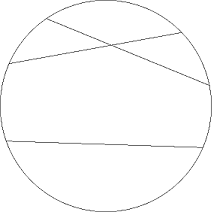
\includegraphics{klein.png}

Эта модель предполагает, что наше пространство на самом деле как бы ограничено, и поэтому в силу именно ограниченности мы можем изобразить какое угодно количество прямых, не пересекающих заданную и проходящих через заданную точку. Единственный сложный вопрос в этой модели в измерении расстояния. При движении к краю окружности масштаб длин должен увеличиваться, чтобы модель удовлетворяла 3 и 4 аксиомам, и одно и то же расстояние в центре диска Клейна и на его краю будет выглядеть сильно по-разному.

Эта модель интересна тем, что она целиком формулируется в терминах геометрии Евклида. То есть модель геометрии Лобачевского получается из непротиворечивости геометрии Евклида: если непротиворечива евклидова геометрия, то непротиворечивой окажется и геометрия Лобачевского, хотя обе они содержат противоречащую друг другу аксиому. Позже выяснилось, что геометрия Лобачевского является не только интересным теоретическим построением но имеет физический смысл: скорости в теории относительности Эйнштейна описываются как раз законами геометрии Лобачевского.

Я к сожалению забыл называние и автора интересной книжки о вымышленном мире, который представлял собой шар в евклидовой геометрии, населенный людьми. Этот шар подчинялся следующему закону: чем ближе человек находился к границе шара, тем меньше он становился по размеру и тем большими для него оказывались расстояния. Эти вымышленные человечки проводили физические эксперименты, и таким образом выяснили, что их вселенная бесконечна и подчиняется законам геометрии Лобачевского. То что на самом деле они живут в евклидовом шаре с особыми свойствами они никаким образом понять не могли.

Как подобный шар и подобные люди могут быть описаны математически мы увидим позже, но сама подобная интерпретация довольно интересна тем, что показывает ограниченность возможности познания: как эти сферические люди ни будут пытаться, они никогда не смогут выяснить что находится за пределами их шара и ничего не узнают о геометрии Евклида, которой на самом деле подчиняется их мир.

Нам же этот пример с геометриями интересен прежде всего тем, что он является хорошей демонстрацией неполноты теории: в абсолютной геометрии утверждение пятой аксиомы является невыводимым, и его можно в результате принять как еще одну аксиому, либо же можно принять как аксиому противоположное утверждение, и оно так же будет непротиворечиво.

Но все сказанное до сих пор относилось лишь к геометрии. Аксиоматизация арифметики натуральных чисел происходила гораздо позднее, чем геометрии, и вплоть до XIX века манипуляции с натуральными числами была неформализованы, и далеко не все видели в такой формализации вообще необходимость. Математик Леопольд Кронекер говорил: «Бог создал натуральные числа, а всё прочее — дело рук человеческих». На сегодняшний день самой известной формализацией (после изложенной мной в этой главе) является система аксиом Пеано, изложенная им в 1889 году в его книге «Принципы арифметики представленные новым методом».

Его аксиомы определяли множество натуральных чисел с помощью константы $0$ и операции инкремента $S$, однако как конкретно выглядят эти константы и операция на языке теории множеств не указывалось, а вместо этого формулировался ряд довольно косвенных свойств, которые были достаточны для определения арифметики:

1) Равенство чисел определялось как отношение эквивалентности.

2) Для любого $n\in\mathbb{N}$ формула $S(n) = 0$ определялась как ложная.

3) $S$ объявлялась инъективной функцией.

4) Оговаривался принцип индукции: если $\phi(0)$ истинно и $\forall n\in\mathbb{N}, \phi(n)\rightarrow \phi(S(n))$, то $\forall n\in\mathbb{N}, \phi(n)$.

Операции сложения и умножения чисел определялись следующим образом:

5) $a+0 = a$

6) $a+S(b) = S(a + b)$

7) $a0 = 0$

8) $aS(b) = ab + a$

Этих аксиом и определений оказывалось достаточным для доказательства всех базовых арифметических свойств.

{\bfseries Упражнение.} Докажите из аксиом Пеано коммутативность умножения $ab=ba$.

Долгое время производились попытки доказать непротиворечивость и полноту аксиом Пеано. Эти попытки были окончательно разбиты в 1931 году, когда Гёдель представил свои теоремы о неполноте. Здесь надо сказать, что Гёдель доказывал теоремы несколько не в том виде и несколько не так, как я представил их в прошлом параграфе. Он был нацелен именно на аксиомы Пеано и использовал в основном аппарат математической логики, а не теории множеств, как это сделал я. Впрочем, у нас не стояло задачи сформулировать максимально строго теорему Гёделя, а лишь понять ее следствия, существенные для большинства математиков.

Для определения натуральных чисел аксиомы Пеано сегодня полностью вытеснены более удобными определениями ZFC. Определение сложения и умножения аксиом Пеано тем не менее осталось довольно полезным, поскольку оно обобщается, и с помощью них  можно удобно определять операции над числами более общего вида, так называемыми ординалами.

ZFC сейчас является базой для 99% всей существующей математики, хотя детали аксиом и правил вывода чаще всего не используются и большинство математиков с ними не знакомы. Вообще основания математики в виде логики и теории множеств существуют довольно отдельно от остальной математики. Терминология теории множеств используется просто как удобный язык, а из логики математики вообще редко прибегают к чему-либо.

Изначально математическая логика развивалась больше как интересное философское направление, позже она постепенно прилаживалась для формализации аксиоматических систем, с развитием компьютерной техники были надежды, что она может стать основой для искусственного интеллекта, но на деле эти надежды оказались сильно преувеличенными. Сейчас математическая логика живет в значительной степени отдельно от остальной математики и какие-то логические результаты лишь изредка вырываются в мир «большой математики». Пожалуй сколько-нибудь значимыми для широких кругов математиков являются лишь рассмотренные в прошлом параграфе теоремы Гёделя, а так же теорема Лёвенгейма-Скулема, которую мы сможем понять лишь позже. Впрочем, даже эти результаты мало кому известны и используются главным образом не сами они, а их следствия.
